\documentclass[11pt, aspectratio= 169]{beamer}
\usetheme{Boadilla}
\setbeamertemplate{caption}[numbered]
\setbeamertemplate{bibliography item}{\insertbiblabel}


\usepackage{amsmath, amssymb}
\usepackage{booktabs, float}
\usepackage{tikz}
\usepackage{graphics}
\graphicspath{{./source/photos}}

\title[Stock returns forecasting]{Neural networks and econometric models in forecasting stock returns}
\author{Andrew~Grishin}

\institute[Faculty of Economics MSU]{Faculty of Economics Moscow State University}
\date{\today}

\begin{document}
	\begin{frame}
		\maketitle
	\end{frame}
	
	\begin{frame}{Agenda}
		\tableofcontents
	\end{frame}
	
	\section{Introduction}
	\begin{frame}{Introduction}
		\begin{columns}
			\begin{column}{0.5\textwidth}
				\centering
				\begin{LARGE}
					\textbf{Reason}
				\end{LARGE}
			\end{column}
			\begin{column}{0.5\textwidth}
				\centering
				\begin{LARGE}
					\textbf{Consequence}
				\end{LARGE}
			\end{column}
		\end{columns}
		\vspace{0.3cm}
		\begin{columns}
			\begin{column}{0.5\textwidth}
				\large
				\begin{itemize}
					\item Money around us
					\item Profit and utility maximization
					\item New methods are needed
					\item How to find the best model in case of different markets?
				\end{itemize}
			\end{column}
			\hspace{0.5cm}
			\begin{column}{0.5\textwidth}
				\large
				\begin{itemize}
					\item Data $\Rightarrow$ Big Data
					\item Statistics $\Rightarrow$ AI \& Econometrics
					\item Machine Learning vs Econometrics
					\item Deep Learning vs Econometrics
				\end{itemize}
			\end{column}
		\end{columns}
	\end{frame}
	
	\subsection{Motivation}
	\begin{frame}{Motivation}
		\Large
		\begin{itemize}
			\item \textbf{Theoretical}: Further rapid development of forecasting models.
			\item \textbf{Practical}: Much easier $\Rightarrow$ much quicker --- "Buy, hold or sell"?
			\item[] As a result --- much reliable decisions $\Rightarrow$ investors are happy.
		\end{itemize}
	\end{frame}
	
	\subsection{Targets}
	\begin{frame}{Targets}
		\Large
		\begin{itemize}
			\item Help traders to make accurate decisions on "Buy, hold or sell"?
			\item Make stock deals more "secure" (low risk) and profitable.
			\item Make people stop being scared of stock market.
		\end{itemize}
	\end{frame}
	
	\subsection{Tasks}
	\begin{frame}{Tasks}
		\Large
		\begin{itemize}
			\item Provide the sequential models’ comparison based on empirical data.
			\item Find the "best" model, according to the topology function.
			\item \textbf{Data}: 15 American and Chinese companies.
			\item[] \textbf{Markets}: Developed (US) and developing (China).
			\item[] \textbf{\textit{NB!}} Various industries (for overall result). 
		\end{itemize}
	\end{frame}
	
	\section{Pre-experiment}
	\subsection{Hypothesis}
	\begin{frame}{Hypothesis}
		\Large
		\textbf{Essential}:
		\begin{itemize}
			\item Market Efficiency \cite{fama1970efficient} - impossible to predict anything.
		\end{itemize}
		
		\textbf{In contrast}:
		\begin{itemize}
			\item Market Fractality \cite{mandelbrot2006misbehavior} - markets have long memory.
			\item Market "inefficiency" \cite{matrin2011history} - Market Efficiency is not true (but best for today).
		\end{itemize}
	
		\textbf{Trial}:
		\begin{itemize}
			\item Neural Network approach is the best for developed and developing markets. 
		\end{itemize}
	\end{frame}
	
	\subsection{Data analysis}
	\begin{frame}{Data analysis}
		\Large
		\begin{itemize}
			\item[] \textbf{What}: Stock prices of 15 US and China companies.
			\item[] \textbf{From}: New York and Shanghai (not Hong-kong) stocks.
			\item[] \textbf{Period}: IPO (different for each company) -- 13/12/2022.
			\item[] \textbf{Industries}: IT (AMD), media (Netflix), sales (Ebay), taxi (Uber), auto (Ford), sport (Nike), energy (General Electric) and so on.
		\end{itemize}
	\end{frame}

	\begin{frame}{Data analysis (visual insights) --- Open prices and returns: US \& China}
		\begin{figure}[H]
			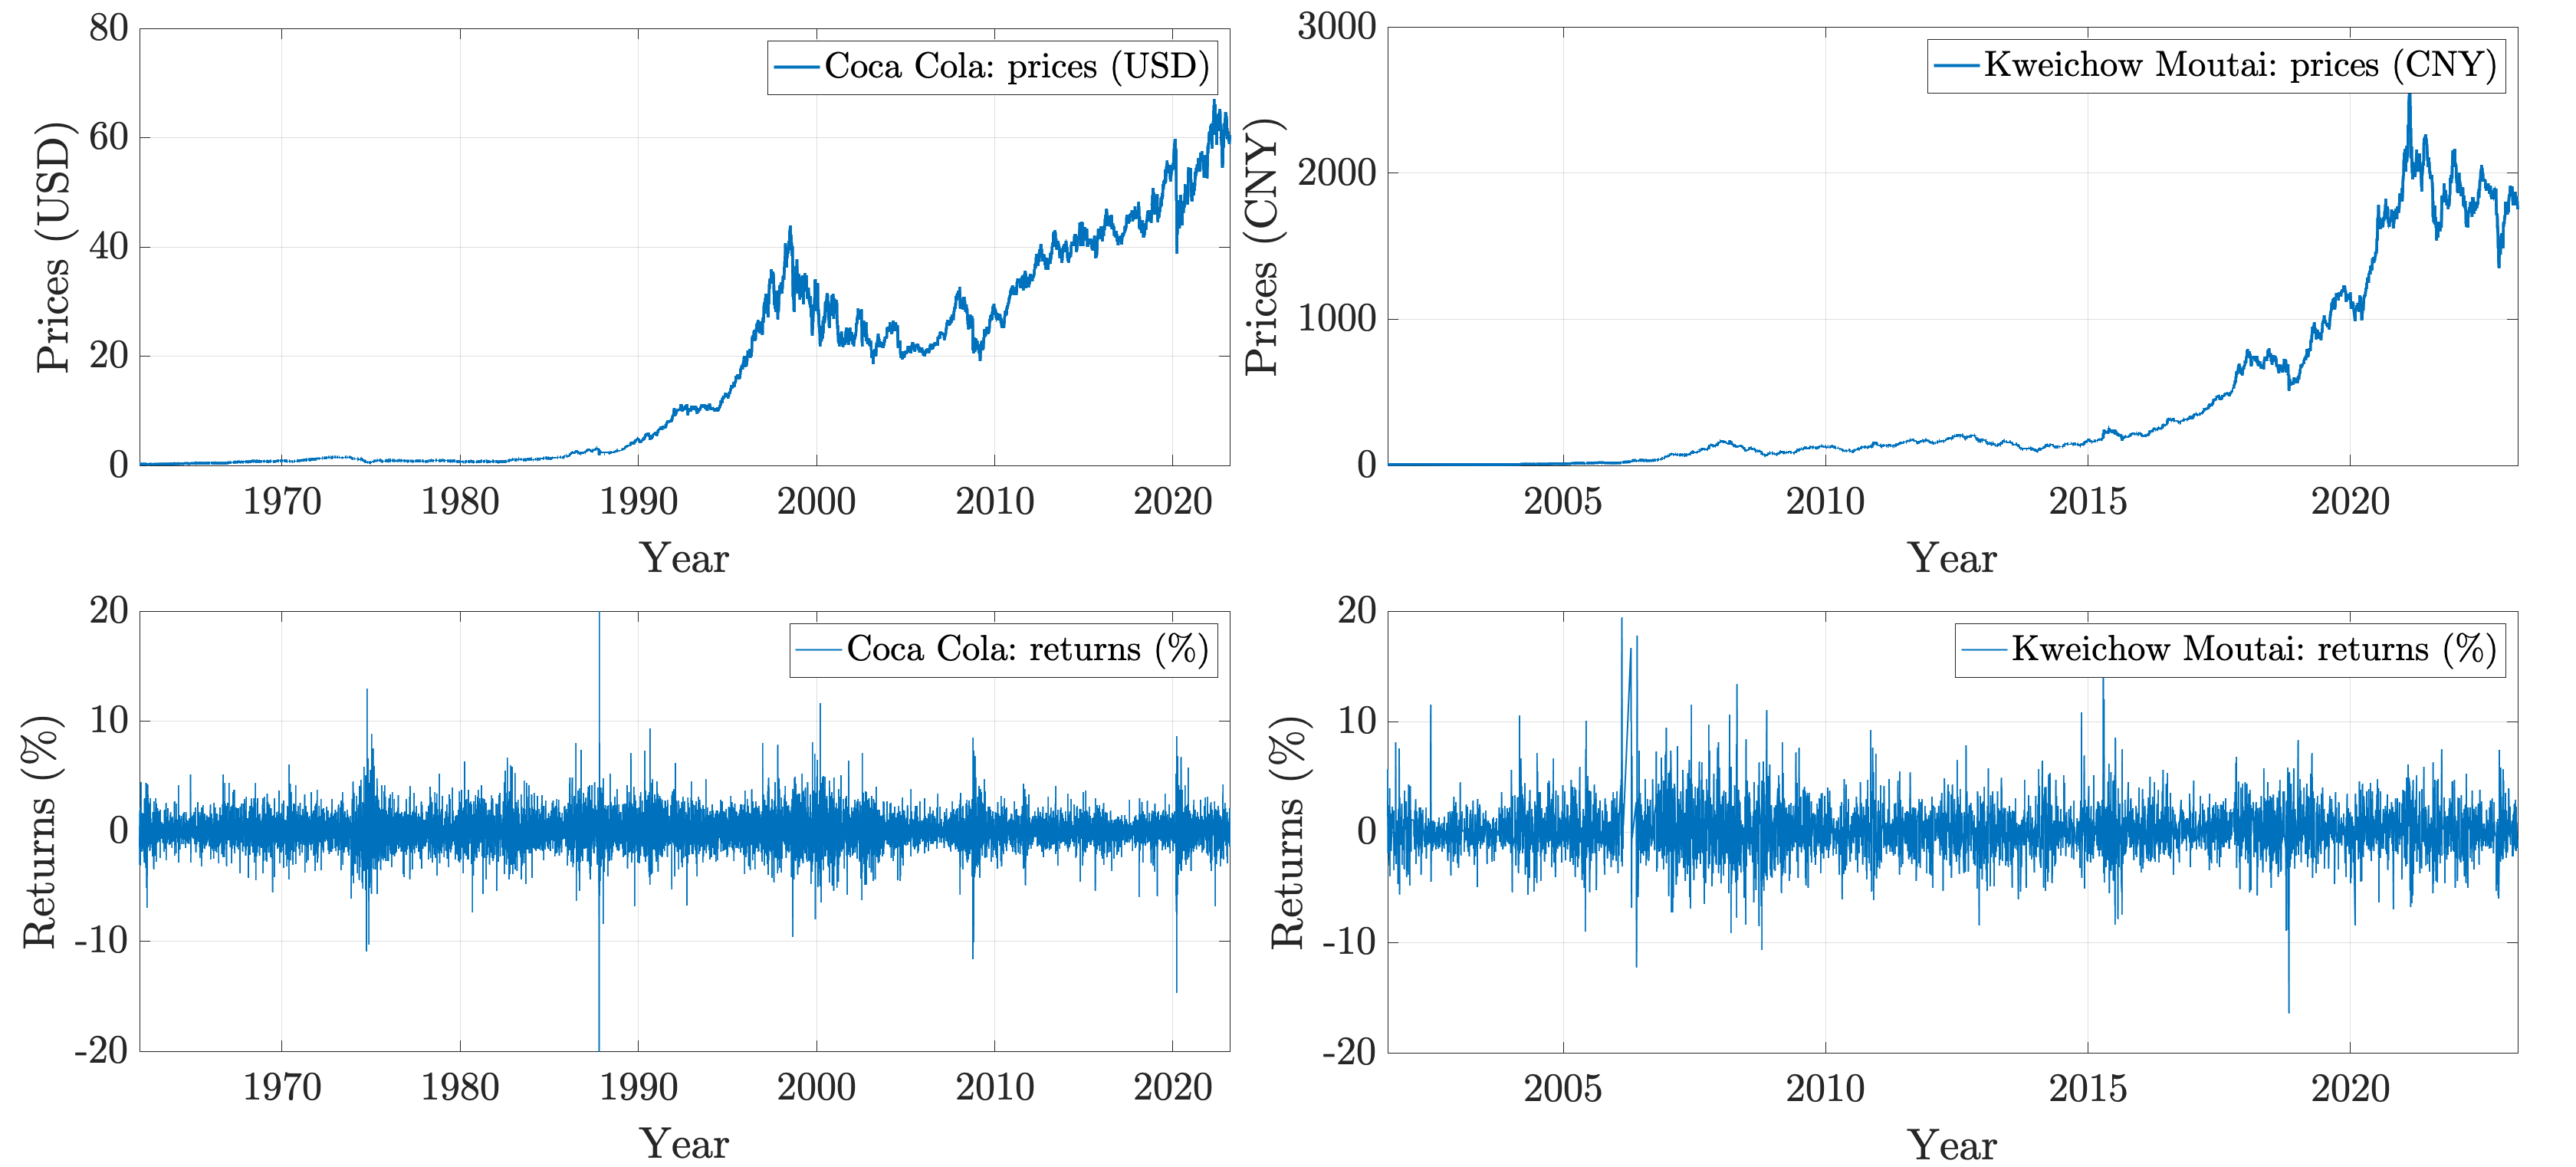
\includegraphics[width= 14cm]{visual_insight.png}
		\end{figure}
	\end{frame}

	\begin{frame}{Data analysis (scalogram insights) --- Coca Cola}
		\begin{figure}[H]
			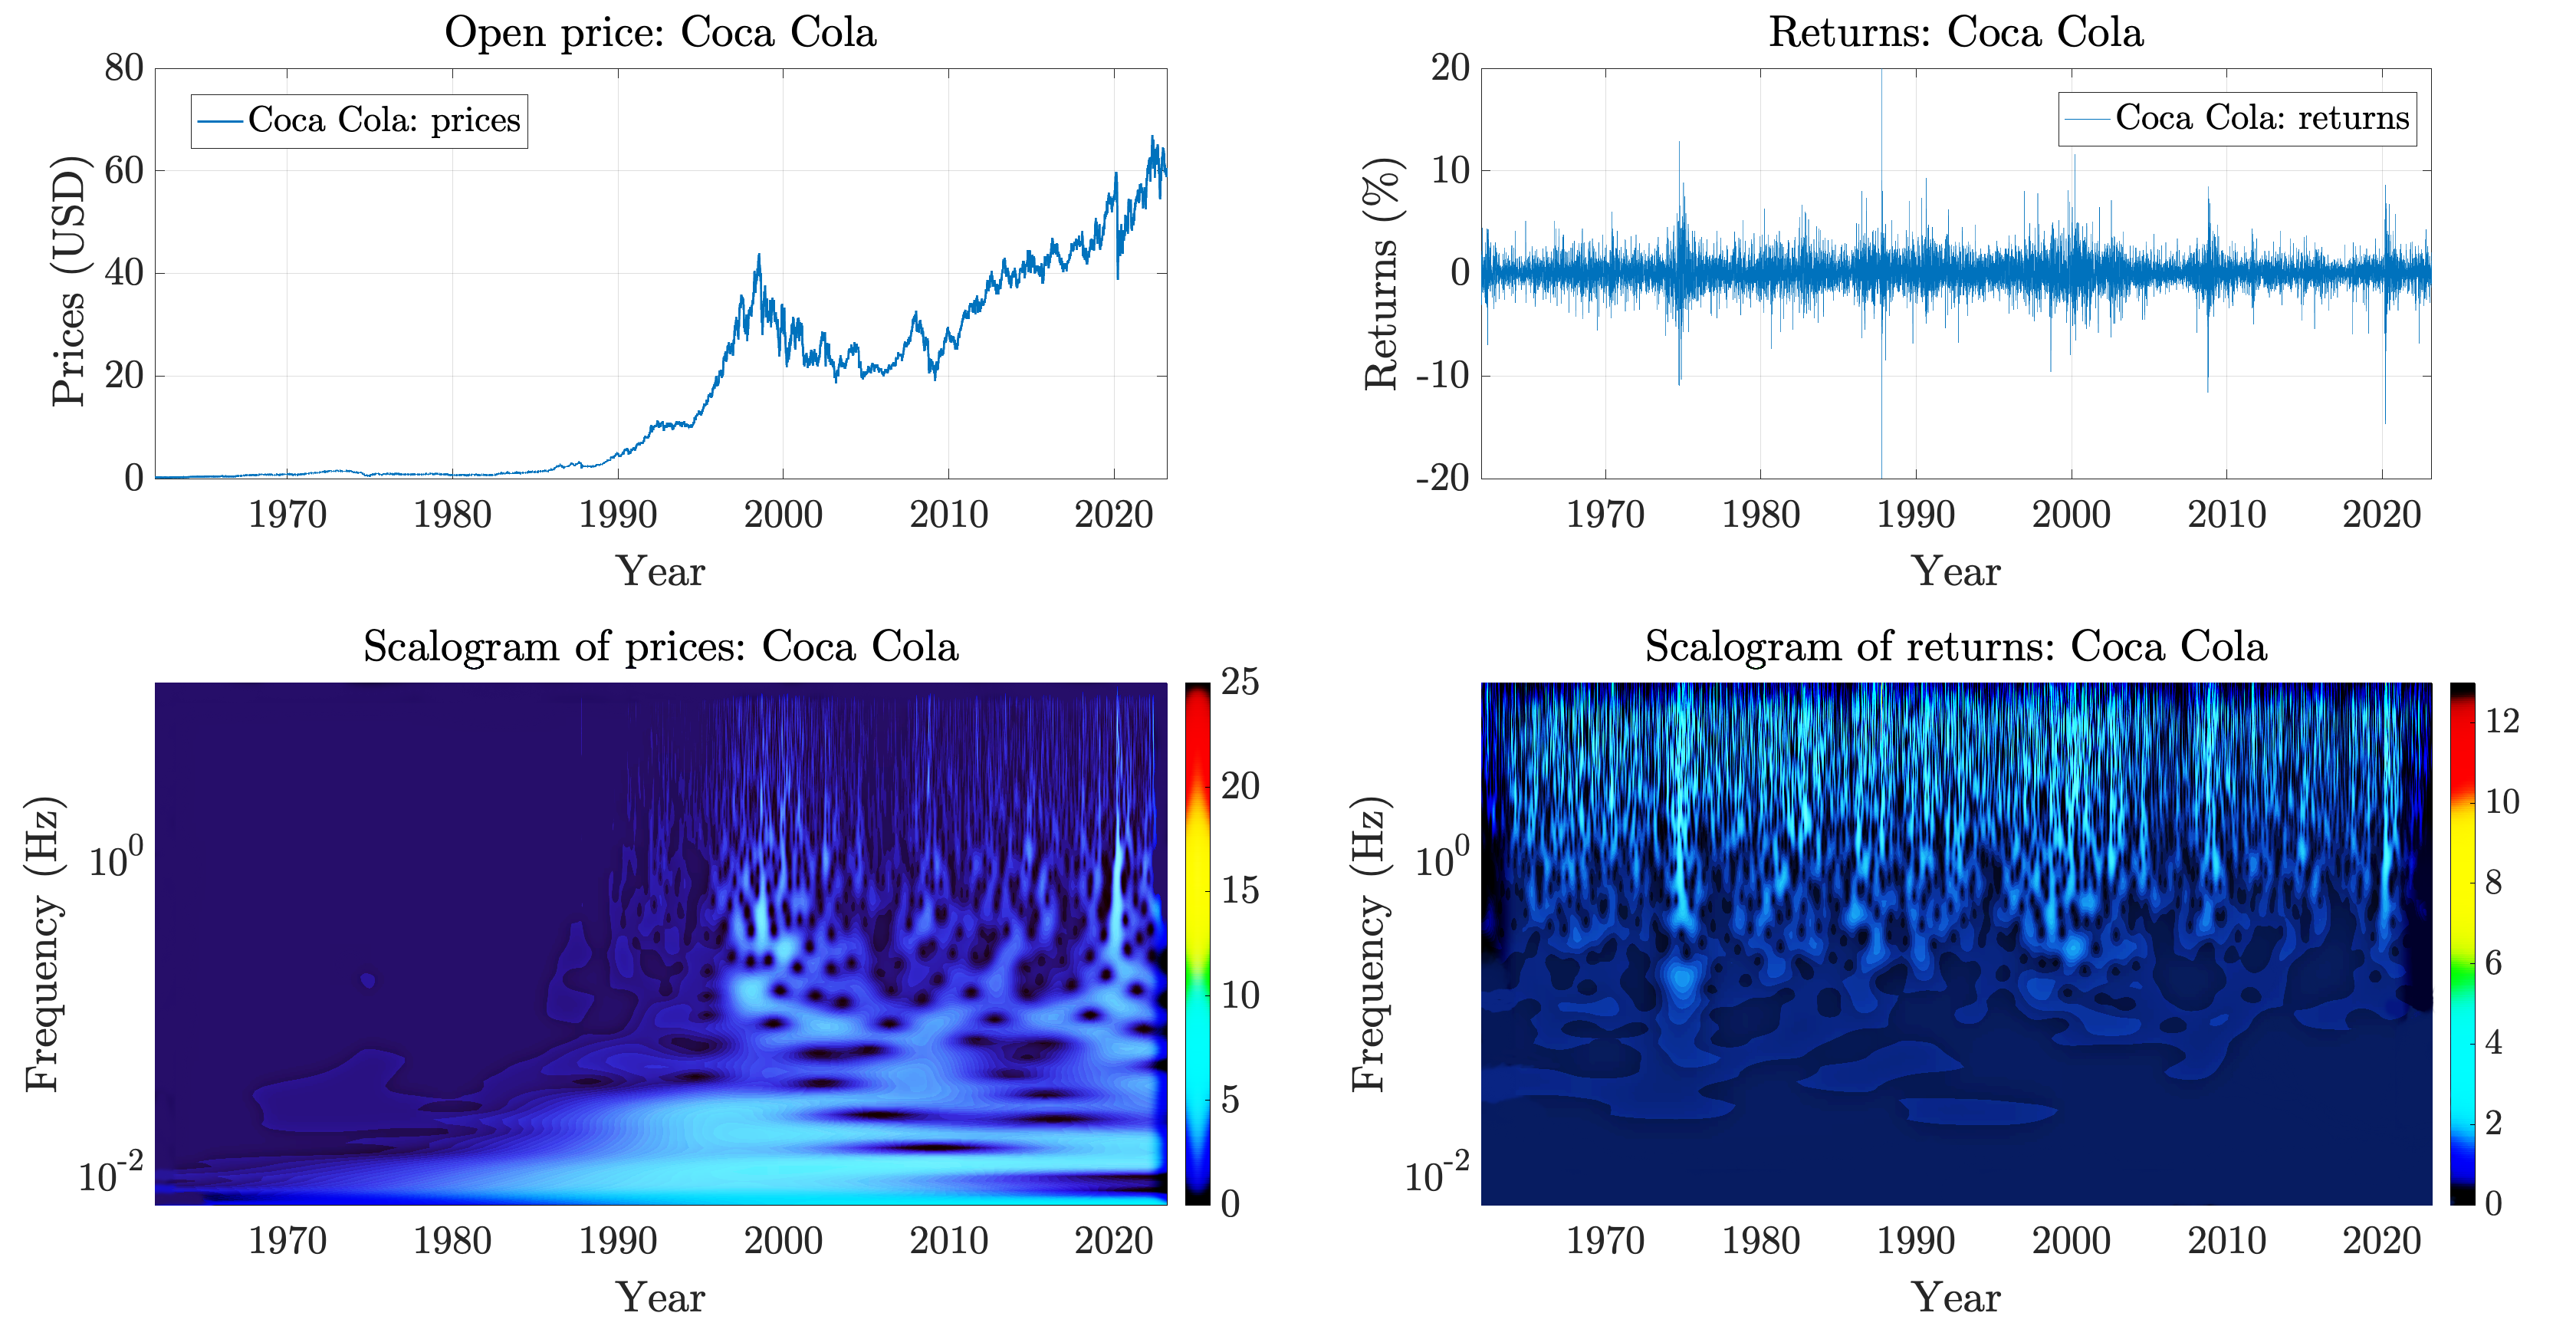
\includegraphics[width= 14cm]{scalogram_insights_us.png}
		\end{figure}
	\end{frame}

	\begin{frame}{Data analysis (scalogram insights): Kweichow Moutai}
		\begin{figure}[H]
			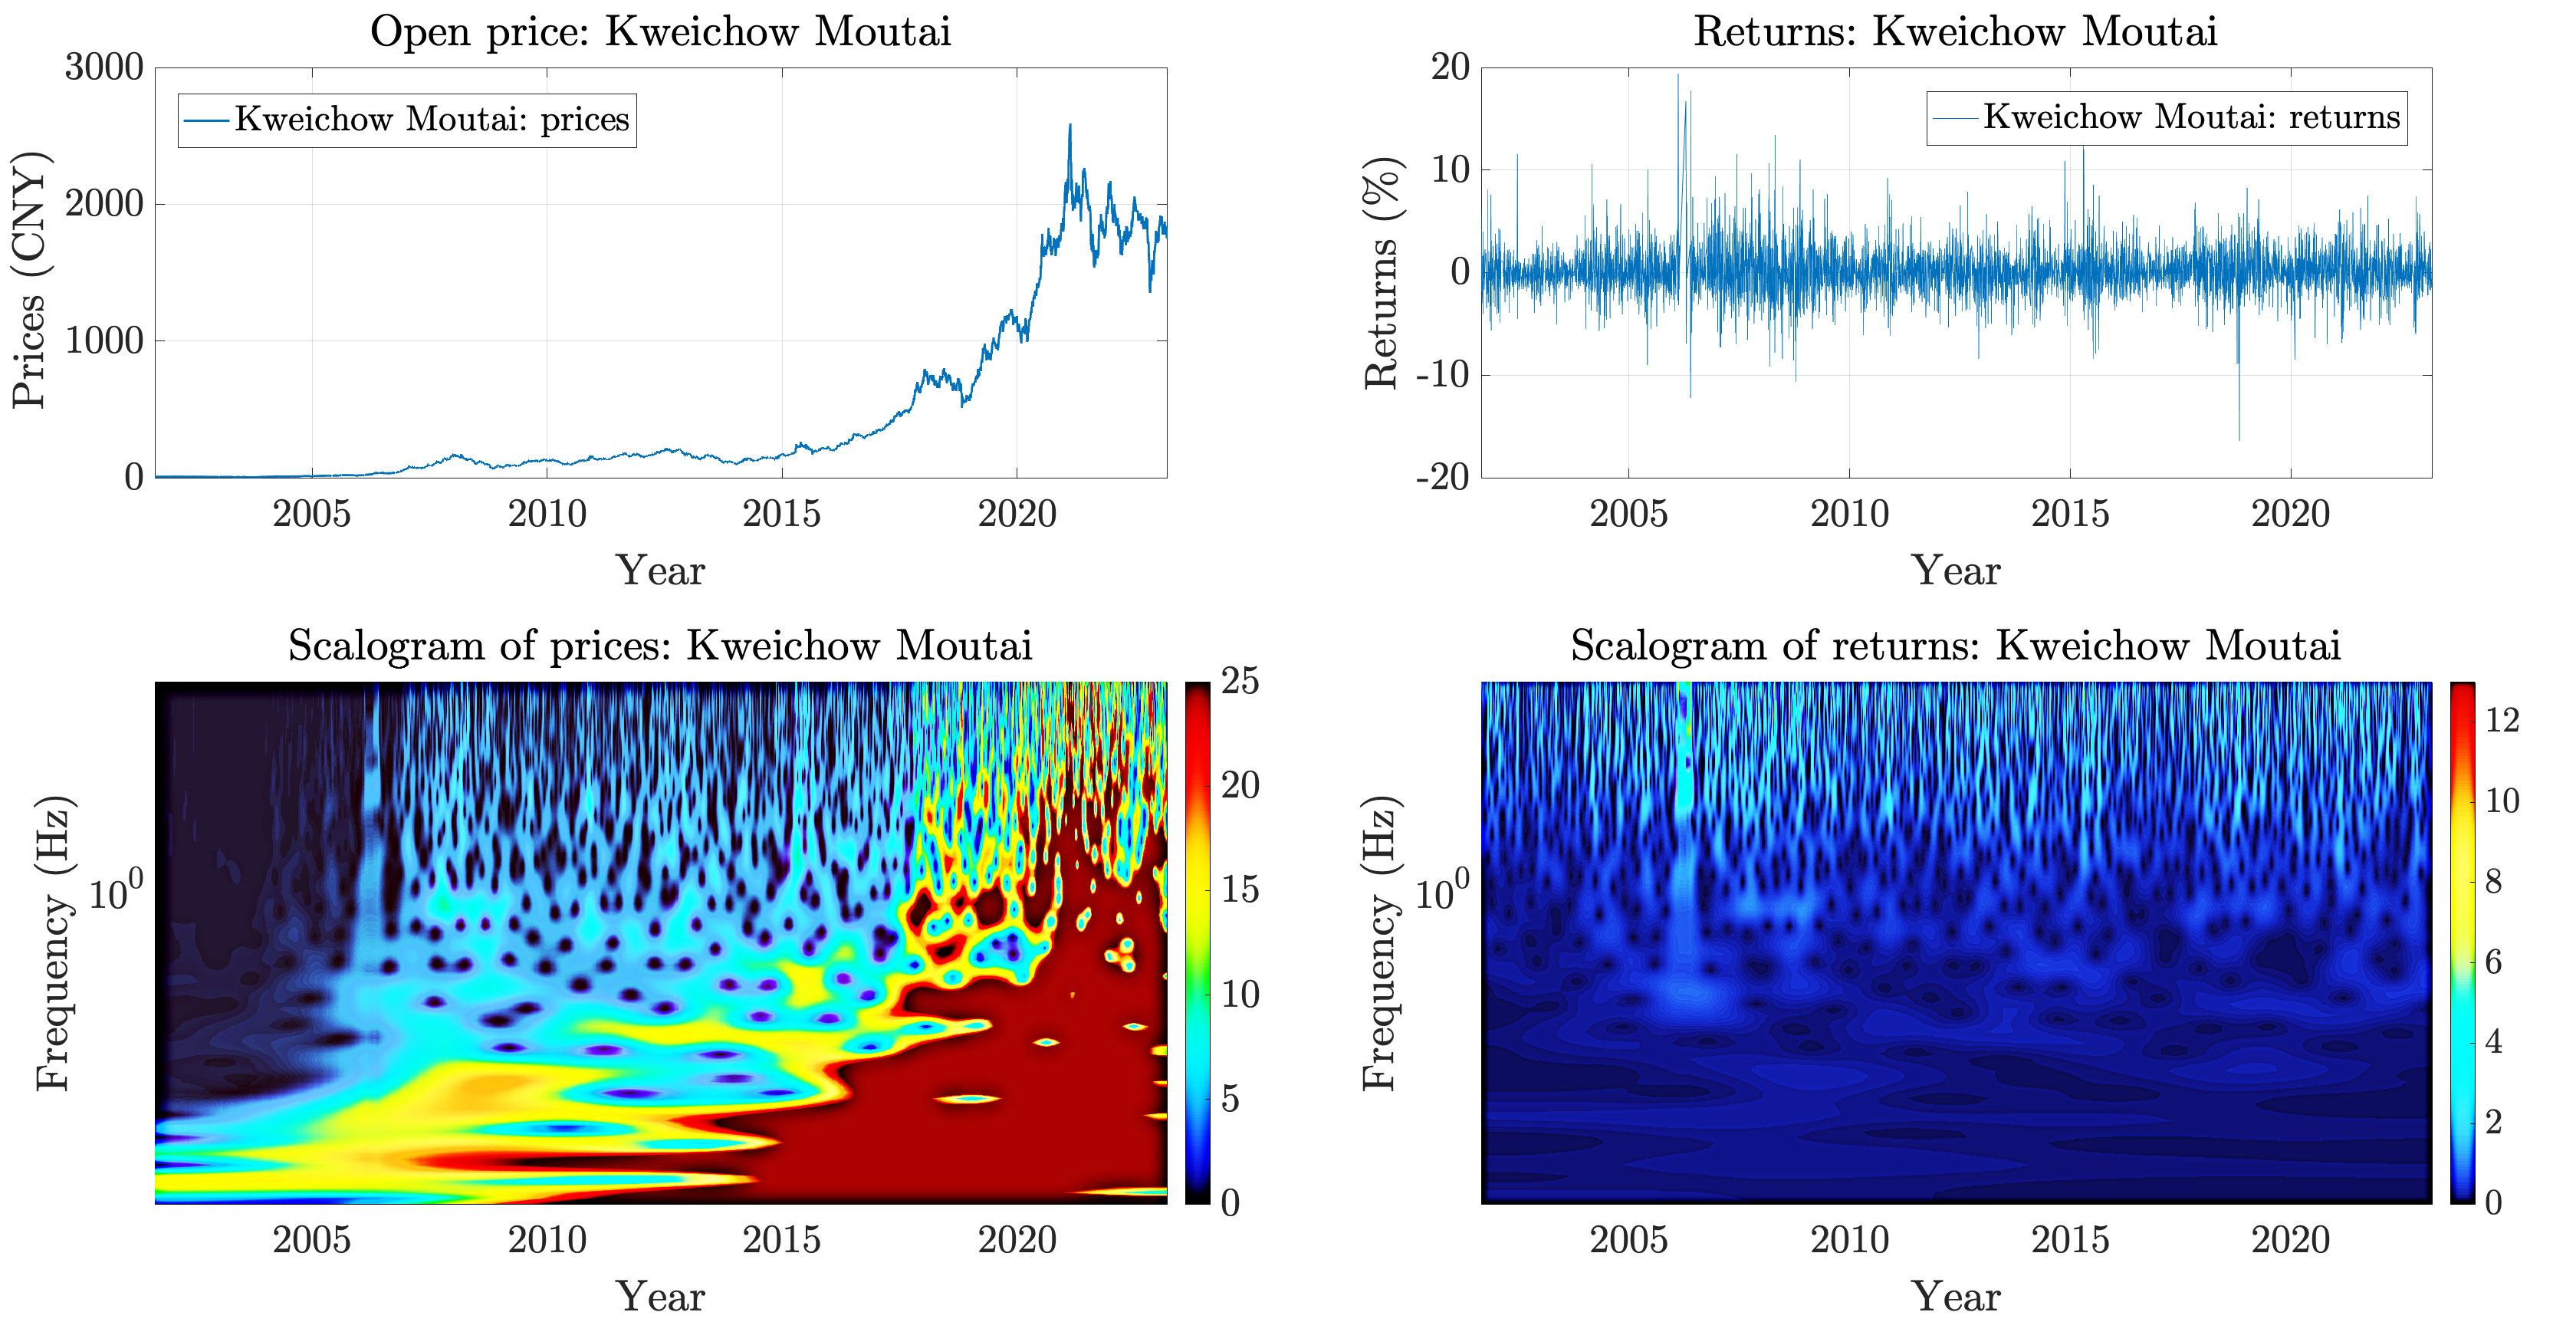
\includegraphics[width= 14cm]{scalogram_insights_china.png}
		\end{figure}
	\end{frame}

	
	\subsection{Method}
	\begin{frame}{Method}
		\begin{columns}
			\begin{column}{0.5\textwidth}
				\textbf{Econometric approach}:
				\begin{center}
					\begin{enumerate}
						\item EWMA
						\item ARIMA
						\item ARIMA + (FI)GARCH
						\item ARFIMA
						\item ARFIMA + (FI)GARCH
						\item SSA (Singular Spectrum Analysis)
					\end{enumerate}
				\end{center}
			\end{column}
			\hfill
			\begin{column}{0.5\textwidth}
				\textbf{Network approach}:
				\begin{center}
					\begin{enumerate}
						\item MLP/RNN/WN
						\item MSSA/EWMA + MLP/RNN/WN
						\item No "transformers" $\Leftarrow$ \cite{zeng2022transformers}
					\end{enumerate}
				\end{center}
				\textbf{Metrics Function}:
				\begin{equation}
					\text{WAPE}(\hat{y}, y) = \frac{\sum_{t= 1}^n |y_t - \hat{y}_t|}{\sum_{t= 1}^n |y_t|}
				\end{equation}
			\end{column}
		\end{columns}
	\end{frame}
	
	\section{Post-experiment}
	\subsection{Tables of comparison}
	\begin{frame}{Tables of comparison}
		content...
	\end{frame}
	
	\subsection{Discussion}
	\begin{frame}{Discussion}
		content...
	\end{frame}
	
	\section{References}
	\begin{frame}{References}
		\bibliographystyle{apalike}
		\bibliography{./source/bibliography/bibliography}
	\end{frame}
	
	\section{Conclusion}
	\begin{frame}{Conclusion}
		\begin{center}
			\LARGE
			Thank you for attention!
		\end{center}
	\end{frame}
\end{document}